\section{How does Design Affect Usability and Learning Done via the App?}\label{sec:future-work-4}

There is a clear connection between design and usability and learning. Here, future work for how design would improve usability or learning is presented.

\subsection{Assessing Coach Guide Knowledge Before the Youth Session}
When asked about the Zambia coach rollout, Josefina points out several challenges. "It feels like some of the coaches forgets the coach guide, even if it has been improved and better integrated with the participant manual. Some of them, don't even use the coach guide." This speaks for that the app should include quizzes for all coach guides as well. When asked if the coach guide quiz are more important than the topic quizzes, she answers that the correct knowledge is more important, because that is the one that needs to be explained correctly to the youth. Therefore, it should be moved into Future work.

\subsection{Using a Flashcards Approach}
In the ideation for iteration 2, flashcards are discussed again, with Henrik Marklund. In iteration 3, this was tested as a lo-fi material with successful results, but more work should be done.

In the ideation of iteration 4, a proposal was given that did not have time to implement. Therefore, the idea is described here: At the coach's second quiz try (having assessed and reflected on the knowledge), flashcards could be introduced to assist the coach in retrieving from memory, before getting the multiple-choice. For future work, when in Training after the first quiz try, The question should be shown \textit{before} the answers are shown, and prompt the coach to think aloud about what they think the answer is, before receiving the alternatives. The coach might be hindered from progressing to the multiple-choice answers until the app has understood the coach has thought hard about their answer to the question.

This is a good use of scaffolding, slowly introducing complicated app features. The hypothesis is inspired from \cite{bjork}, that knowledge is strengthened if the coach retrieves from memory, versus looking up the answer or choosing the most likely answer.

\subsection{Adding more media channels to more closely simulate the learning environment}
To simulate the entrepreneur coach environment more accurately could possibly increase memorization of procedural learning objectives. Research exists that supports how using multiple channels like audio, video, voice could be beneficial, or to use interactive simulations.  The advantage of multiple-choice from a developer perspective is that data can be collected easily and because of ease of implementation. From YoungDrive's perspective, it serves the target group of the coaches being first-time smartphone users well \citep{youngdrive-masterthesis-idea}.

\subsection{Improvements to the Certification Mode}

Following the advice from \cite{sierra} of quickly giving the user a feeling of a superpower, this should be becoming a Certified coach in the future. From the end results of iteration 4, we can learn that notably the intrinsic motivation is high, deliberate practice is present, and the coach can feel the intrinsic reward of having pushed herself and learned the material when certified. This is very positive.

This reaction, could and should be even more amplified when certified. It is discussable if this should be done by simple gamification, but an opinion by a coach was that medals earned should be more visible and that sounds could strengthen the feeling of achievement. Also, the quiz list could show these results, increasing motivation to take other quizzes that you have not yet mastered, or to better your score in a topic where you had not become certified.

\subsection{Improvements training Correct Structure and Time Management}
During all app tests (iteration 2-4), it has been shown that since Correct Structure and Time Management are both ordinal, the Training mode for such topics would be more suitable as interactive exercises than multiple-choice. The proposal is to first use drag-and-drop to place each activity of a youth session in the correct order, and then selecting the right time for the each activity. This assists the coach in creating a mental model, which can be used to retrieve from memory during the assessment.

\subsection{Scaffolding with Flashcards}
After the coach's first new try, Flashcards could be introduced to assist the coach in retrieving in memory, before getting the multiple-choice. To do this after the first assessment, is partly because of technology scaffolding (introduce new concepts in steps), partly because the knowledge is strengthened if the coach retrieves from memory versus looking up the answer or choosing the most likely answer \citep{bjork}.

\subsection{Memory Design}
For the ideation of iteration 4, it was pointed out by pedagogical expert Henrik Marklund that if knowledge is to be memorized, memory techniques could be used. One such e-learning tool is \cite{memorize}. The tool has interactive learning modes, aiming to learn facts and terms with speed. This was not prioritized because of time constraints working with technical features that were not essential. Also, the idea was never proposed by users, only by experts. Moreover, the teacher opposed the idea of remembering answers that were not in the factual remember category. To do so, would oppose the learning objectives, which score higher on Bloom's revised taxonomy. However, to study how the coaches can remember better via an app, and learn memory techniques via the app, could be a future work which is advisable.

\subsection{Sharing with One Another}

In future versions of the app, mechanics of sharing content and co-creation would add value connected to Bloom's, reaching Create and Apply. Adding these game elements goes in line with Clark's research, which showed a positive correlation with learning and games that required multi-player collaboration \citep{gates}.


\subsection{Including the Paper Manuals in the App}

Already in iteration 2, it was proposed by coaches if the participant manual and coach guide could be included in the app, instead of as paper. The teacher agreed in principle, especially as the paper coach guide is often overlooked (reading the digital version could be designed to be made mandatory before unlocking other features), but also saw several challenges.  Because of broadband limitations the manuals would take a lot of space to download. Also, the manuals are designed in A4 format, while a smartphone screen or even tablet is much smaller, making it cumbersome to read the whole manuals in the same way you would with the paper versions.

However, for the ideation of iteration 3, it was realized that if the manuals could be converted into smaller chunks, there is an opportunity for bite-sized spaced learning, instead of massed learning. How to split the manuals into these small parts? Well, by extracting the important parts for understanding an answer to a specific question, see figure \ref{fig:bite-size}. The teacher emphasised that this would take time for her to do, but that the effort would be worth it. While there were no time for including the whole manuals, there was an idea the teacher thought acceptable for iteration 4: including on which page the coach would find the answer to a specific question. This was not one of the most prioritized features of iteration 4, which it was never done, but for further work, this should be investigated.

\begin{figure}[h]
    \centering
    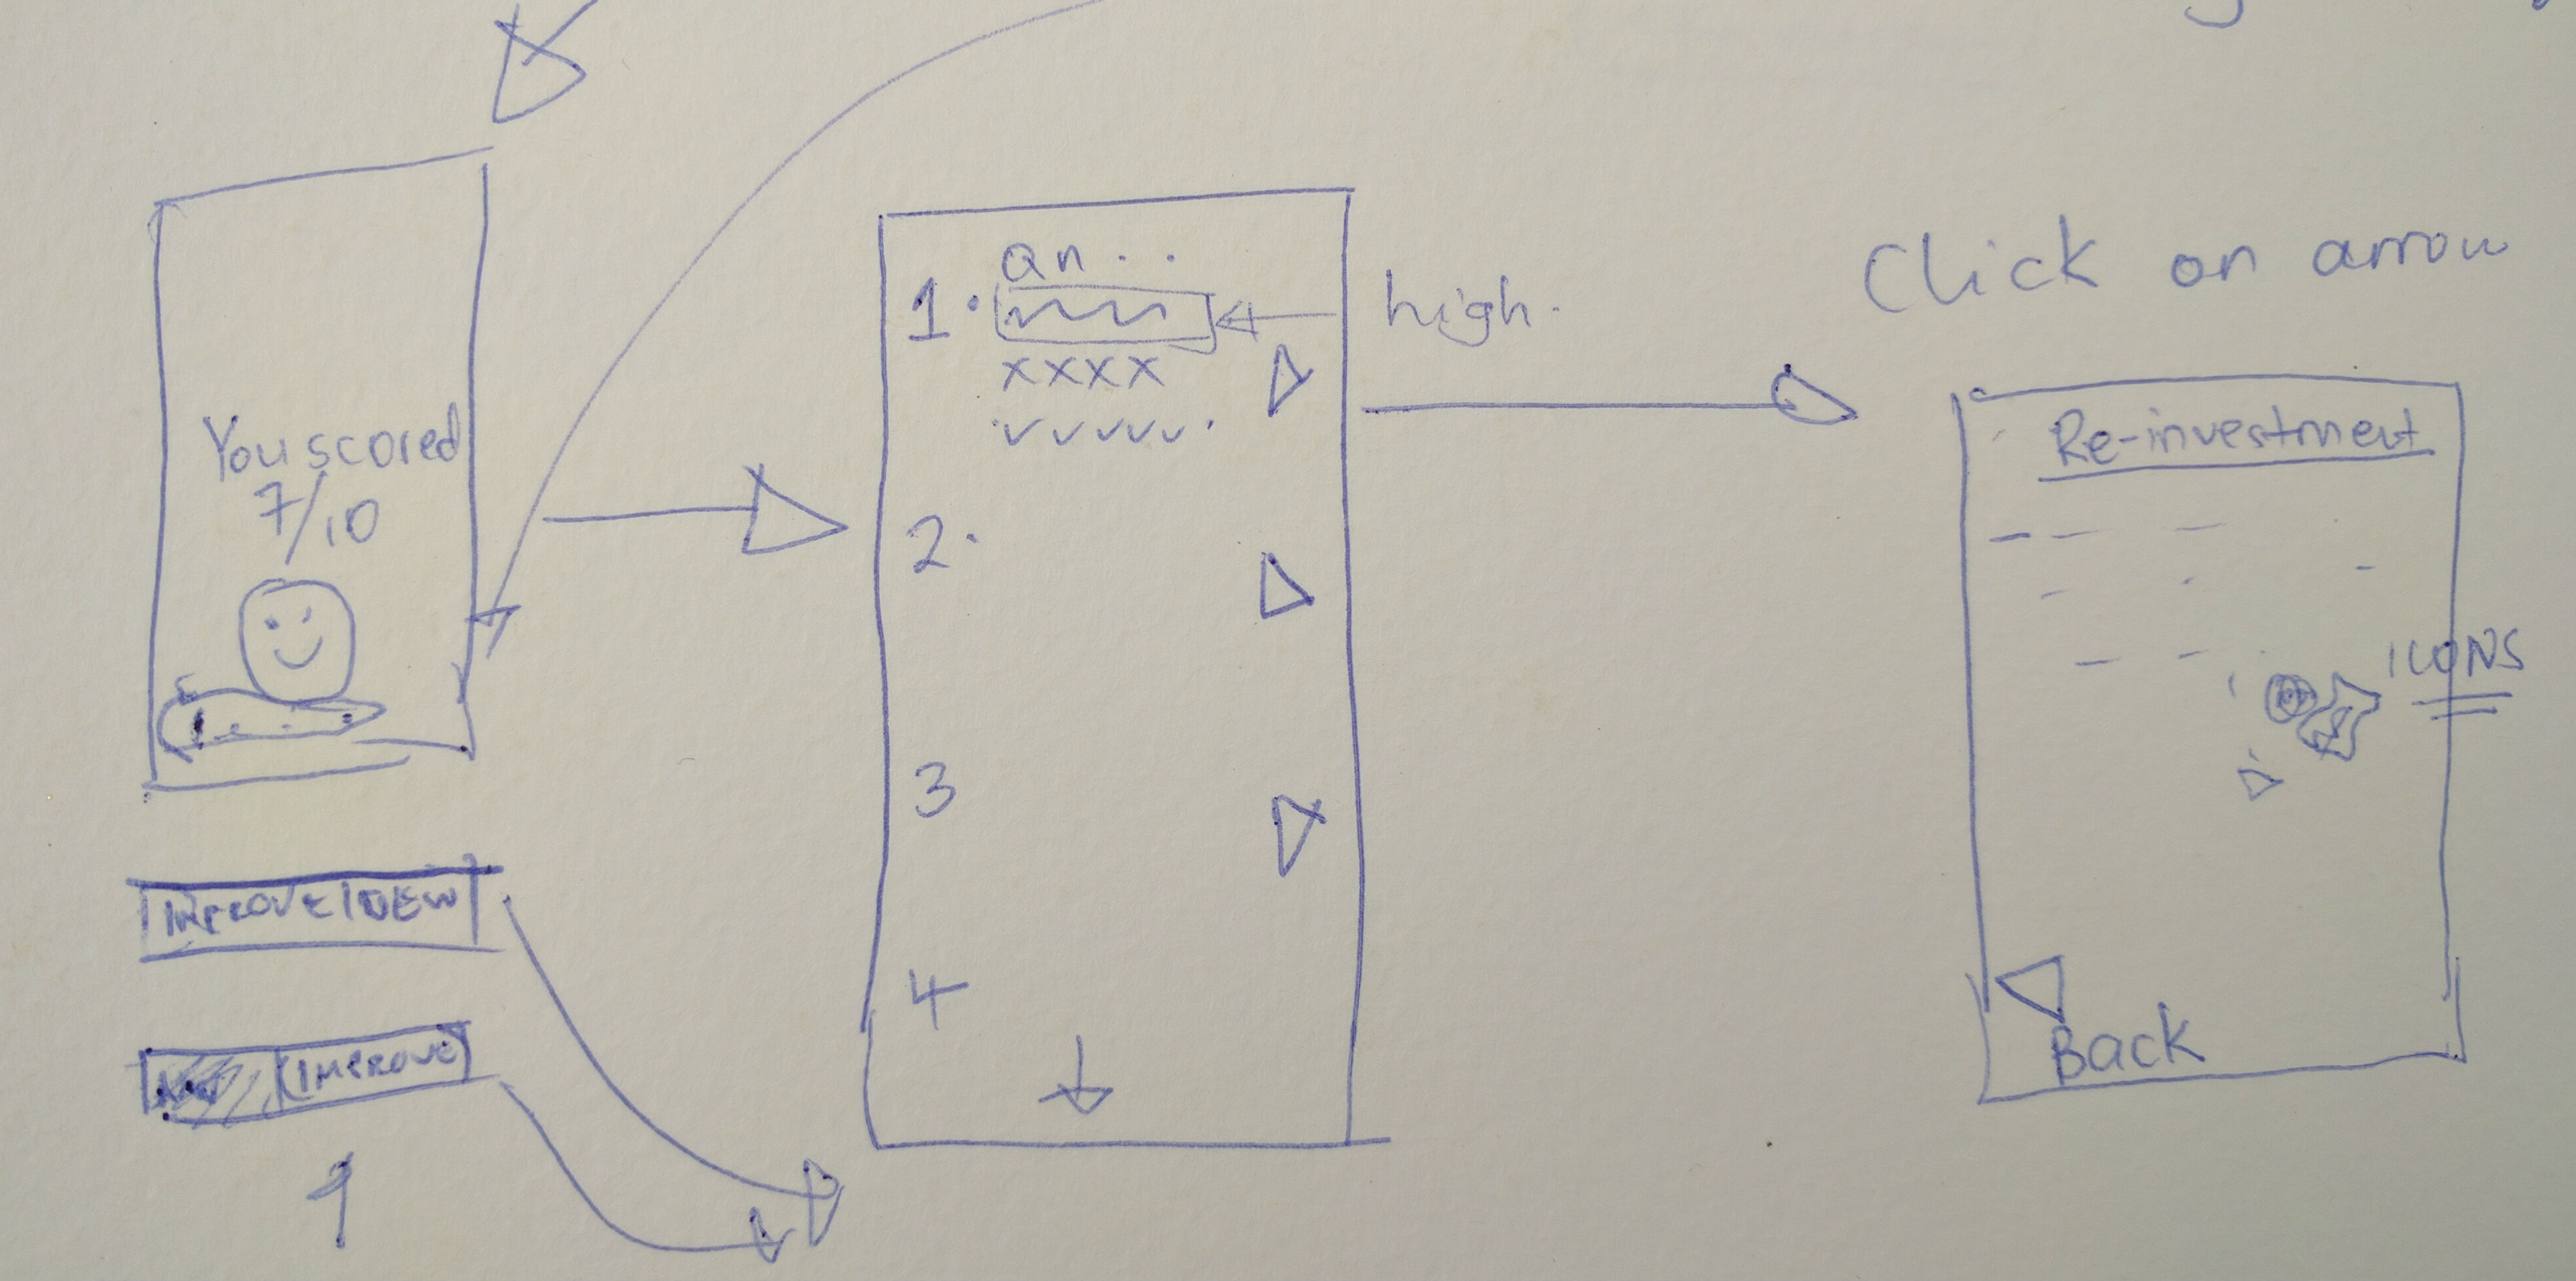
\includegraphics[width=0.8\textwidth]{biteSize.jpg}
    %IterationProcess.png
    \caption{By clicking on an arrow next to the question showing the correct answer compared with your answer, the coach could read an extract from the YoungDrive manuals, which includes the right answer. The learning benefit compared to just observing the right answer, is that the coach gets the answer in context, which improves memorization and understanding. An idea would be to no longer give the coach the correct answer in the score board, but to instead let the coach choose the right answer after reading the text.}
    \label{fig:bite-size}
\end{figure}

A major opportunity doing this would be to replace the paper manuals. Today, the manuals are the most expensive post of YoungDrive, which is why this would be attractive. While a smartphone or tablet could be returned after a YoungDrive program has ended, this is not possible with the paper versions, so there might be a monetary incentive to do so. A problem that would need to be addressed is that the manuals also have written exercises in them. These exercises could be made interactive in the app, which would also allowed for smart features such as automatic assessment, financial literacy simulations, etcetera. While this was not a scope of the master thesis, it is interesting further work to test if such interactive exercises and simulations would be effective in the developing country context of learning and teaching entrepreneurship.
